%%%%%%%%%%%%%%%%%%%%%%%%%%%%%%%%%%%%%%%%%%%%%%%%%%%%%%%%%%%%%%%%%%%%%%%%%%%%%%%%%%%%
% Template for STAT 547C final project
% Author: Ben Bloem-Reddy <benbr@stat.ubc.ca>
% Date: Oct. 18, 2019
%%%%%%%%%%%%%%%%%%%%%%%%%%%%%%%%%%%%%%%%%%%%%%%%%%%%%%%%%%%%%%%%%%%%%%%%%%%%%%%%%%%%

% Note: You will get an empty bibliography warning when compiling until you include a citation.

\documentclass[10pt]{article}
% header.tex
% this is where you load pacakges, specify custom formats, etc.

\usepackage[left=1in,right=1in,top=0.75in,footskip=25pt]{geometry} 
% \usepackage{changepage}
\usepackage{amsmath,amsthm,amssymb,amsfonts}
\usepackage{mathtools}
% enumitem for custom lists
\usepackage{enumitem}
% Load dsfont this to get proper indicator function (bold 1) with \mathds{1}:
\usepackage{dsfont}
\usepackage{centernot}

\usepackage[usenames,dvipsnames]{xcolor}

% set up commenting code (I will use this during marking)
\definecolor{CommentColor}{rgb}{0,.50,.50}
\newcounter{margincounter}
\newcommand{\displaycounter}{{\arabic{margincounter}}}
\newcommand{\incdisplaycounter}{{\stepcounter{margincounter}\arabic{margincounter}}}
\newcommand{\COMMENT}[1]{\textcolor{CommentColor}{$\,^{(\incdisplaycounter)}$}\marginpar{\scriptsize\textcolor{CommentColor}{ {\tiny $(\displaycounter)$} #1}}}

\usepackage{appendix}

% set up graphics
\usepackage{graphicx}
\DeclareGraphicsExtensions{.pdf,.png,.jpg}
\graphicspath{ {fig/} }

\usepackage[sorting=nyt,backend=biber,bibstyle=alphabetic,citestyle=alphabetic,giveninits=true]{biblatex}

\usepackage{fancyhdr}
\pagestyle{fancy}
\setlength{\headheight}{40pt}

%%%%%%%%%%%%%%%%%%%%%%%%%%%%%%%%%%%%%%%%%%%%%%%%%%%%%%%%%%%%%%%%%%%%%%%%%%%%%%%%%%%%
% most other packages you might use should be loaded before hyperref
%%%%%%%%%%%%%%%%%%%%%%%%%%%%%%%%%%%%%%%%%%%%%%%%%%%%%%%%%%%%%%%%%%%%%%%%%%%%%%%%%%%%

% Set up hyperlinks:
\definecolor{RefColor}{rgb}{0,0,.65}
\usepackage[colorlinks,linkcolor=RefColor,citecolor=RefColor,urlcolor=RefColor]{hyperref}

\usepackage[capitalize]{cleveref}
\crefname{appsec}{Appendix}{Appendices} % you can tell cleveref what to call things
% defs.tex
% this is where you define custom notation, commands, etc.


%%
% full alphabets of different styles
%%

% bf series
\def\bfA{\mathbf{A}}
\def\bfB{\mathbf{B}}
\def\bfC{\mathbf{C}}
\def\bfD{\mathbf{D}}
\def\bfE{\mathbf{E}}
\def\bfF{\mathbf{F}}
\def\bfG{\mathbf{G}}
\def\bfH{\mathbf{H}}
\def\bfI{\mathbf{I}}
\def\bfJ{\mathbf{J}}
\def\bfK{\mathbf{K}}
\def\bfL{\mathbf{L}}
\def\bfM{\mathbf{M}}
\def\bfN{\mathbf{N}}
\def\bfO{\mathbf{O}}
\def\bfP{\mathbf{P}}
\def\bfQ{\mathbf{Q}}
\def\bfR{\mathbf{R}}
\def\bfS{\mathbf{S}}
\def\bfT{\mathbf{T}}
\def\bfU{\mathbf{U}}
\def\bfV{\mathbf{V}}
\def\bfW{\mathbf{W}}
\def\bfX{\mathbf{X}}
\def\bfY{\mathbf{Y}}
\def\bfZ{\mathbf{Z}}

% bb series
\def\bbA{\mathbb{A}}
\def\bbB{\mathbb{B}}
\def\bbC{\mathbb{C}}
\def\bbD{\mathbb{D}}
\def\bbE{\mathbb{E}}
\def\bbF{\mathbb{F}}
\def\bbG{\mathbb{G}}
\def\bbH{\mathbb{H}}
\def\bbI{\mathbb{I}}
\def\bbJ{\mathbb{J}}
\def\bbK{\mathbb{K}}
\def\bbL{\mathbb{L}}
\def\bbM{\mathbb{M}}
\def\bbN{\mathbb{N}}
\def\bbO{\mathbb{O}}
\def\bbP{\mathbb{P}}
\def\bbQ{\mathbb{Q}}
\def\bbR{\mathbb{R}}
\def\bbS{\mathbb{S}}
\def\bbT{\mathbb{T}}
\def\bbU{\mathbb{U}}
\def\bbV{\mathbb{V}}
\def\bbW{\mathbb{W}}
\def\bbX{\mathbb{X}}
\def\bbY{\mathbb{Y}}
\def\bbZ{\mathbb{Z}}

% cal series
\def\calA{\mathcal{A}}
\def\calB{\mathcal{B}}
\def\calC{\mathcal{C}}
\def\calD{\mathcal{D}}
\def\calE{\mathcal{E}}
\def\calF{\mathcal{F}}
\def\calG{\mathcal{G}}
\def\calH{\mathcal{H}}
\def\calI{\mathcal{I}}
\def\calJ{\mathcal{J}}
\def\calK{\mathcal{K}}
\def\calL{\mathcal{L}}
\def\calM{\mathcal{M}}
\def\calN{\mathcal{N}}
\def\calO{\mathcal{O}}
\def\calP{\mathcal{P}}
\def\calQ{\mathcal{Q}}
\def\calR{\mathcal{R}}
\def\calS{\mathcal{S}}
\def\calT{\mathcal{T}}
\def\calU{\mathcal{U}}
\def\calV{\mathcal{V}}
\def\calW{\mathcal{W}}
\def\calX{\mathcal{X}}
\def\calY{\mathcal{Y}}
\def\calZ{\mathcal{Z}}


%%%%%%%%%%%%%%%%%%%%%%%%%%%%%%%%%%%%%%%%%%%%%%%%%%%%%%%%%%
% text short-cuts
\def\iid{i.i.d.\ } %i.i.d.
\def\ie{i.e.\ }
\def\eg{e.g.\ }
\def\Polya{P\'{o}lya\ }
%%%%%%%%%%%%%%%%%%%%%%%%%%%%%%%%%%%%%%%%%%%%%%%%%%%%%%%%%%

%%%%%%%%%%%%%%%%%%%%%%%%%%%%%%%%%%%%%%%%%%%%%%%%%%%%%%%%%%
% quasi-universal probabilistic and mathematical notation
% my preferences (modulo publication conventions, and clashes like random vectors):
%   vectors: bold, lowercase
%   matrices: bold, uppercase
%   operators: blackboard (e.g., \mathbb{E}), uppercase
%   sets, spaces: calligraphic, uppercase
%   random variables: normal font, uppercase
%   deterministic quantities: normal font, lowercase
%%%%%%%%%%%%%%%%%%%%%%%%%%%%%%%%%%%%%%%%%%%%%%%%%%%%%%%%%%

% operators
\def\P{\bbP} %fundamental probability
\def\E{\bbE} %expectation
% conditional expectation
\DeclarePairedDelimiterX\bigCond[2]{[}{]}{#1 \;\delimsize\vert\; #2}
\newcommand{\conditional}[3][]{\bbE_{#1}\bigCond*{#2}{#3}}
\def\Law{\mathcal{L}} %law; this is by convention in the literature
\def\indicator{\mathds{1}} % indicator function

% sets and groups
\def\borel{\calB} %Borel sets
\def\sigAlg{\calA} %sigma-algebra
\def\filtration{\calF} %filtration
\def\grp{\calG} %group

% binary relations
\def\condind{{\perp\!\!\!\perp}} %independence/conditional independence
\def\equdist{\stackrel{\text{\rm\tiny d}}{=}} %equal in distribution
\def\equas{\stackrel{\text{\rm\tiny a.s.}}{=}} %euqal amost surely
\def\simiid{\sim_{\mbox{\tiny iid}}} %sampled i.i.d

% common vectors and matrices
\def\onevec{\mathbf{1}}
\def\iden{\mathbf{I}} % identity matrix
\def\supp{\text{\rm supp}}

% misc
% floor and ceiling
\DeclarePairedDelimiter{\ceilpair}{\lceil}{\rceil}
\DeclarePairedDelimiter{\floor}{\lfloor}{\rfloor}
\newcommand{\argdot}{{\,\vcenter{\hbox{\tiny$\bullet$}}\,}} %generic argument dot
%%%%%%%%%%%%%%%%%%%%%%%%%%%%%%%%%%%%%%%%%%%%%%%%%%%%%%%%%%

%%%%%%%%%%%%%%%%%%%%%%%%%%%%%%%%%%%%%%%%%%%%%%%%%%%%%%%%%%
%% some distributions
% continuous
\def\UnifDist{\text{\rm Unif}}
\def\BetaDist{\text{\rm Beta}}
\def\ExpDist{\text{\rm Exp}}
\def\GammaDist{\text{\rm Gamma}}
% \def\GenGammaDist{\text{\rm GGa}} %Generalized Gamma

% discrete
\def\BernDist{\text{\rm Bernoulli}}
\def\BinomDist{\text{\rm Binomial}}
\def\PoissonPlus{\text{\rm Poisson}_{+}}
\def\PoissonDist{\text{\rm Poisson}}
\def\NBPlus{\text{\rm NB}_{+}}
\def\NBDist{\text{\rm NB}}
\def\GeomDist{\text{\rm Geom}}
% \def\CRP{\text{\rm CRP}}
% \def\EGP{\text{\rm EGP}}
% \def\MittagLeffler{\text{\rm ML}}
%%%%%%%%%%%%%%%%%%%%%%%%%%%%%%%%%%%%%%%%%%%%%%%%%%%%%%%%%%

%%%%%%%%%%%%%%%%%%%%%%%%%%%%%%%%%%%%%%%%%%%%%%%%%%%%%%%%%%
% Project-specific notation should go here
% (Because it's at the end of the file, it can overwrite anything that came before.)

%e.g.,
\def\Laplacian{\calL}
\def\P{\calP}

% combinatorial objects
\def\perm{\sigma} %fixed permutation
\def\Perm{\Sigma} %random permutation
\def\part{\pi} %fixed partition
\def\Part{\Pi} %random partition


%%%%%%%%%%%%%%%%%%%%%%%%%%%%%%%%%%%%%%%%%%%%%%%%%%%%%%%%%%
\usepackage{booktabs}
\usepackage{bbm}
\usepackage{amsmath,amsthm,amssymb,amsfonts}
\newtheorem{theorem}{Theorem}
\newtheorem{corollary}{Corollary}
\newtheorem{lemma}{Lemma}
\newtheorem{example}{Example}
\newtheorem{definition}{Definition}
\newtheorem{exercise}{Exercise}


%%%%%%%%%%%%%%%%%%%%%%%%%%%%%%%%%%%%%%%%%%%%%%%%%%%%%%%%%%%%%%%%%%%%%%%%%%%%%%%%%

% your title/author/date information go here
\title{Martingale Convergence Theorem and Stochastic Optimization} % replace with your title
\author{Grace Yin} % replace with your name
\date{\today} % replace with your submission date

\bibliography{../../ref/STAT_547C.bib} % add the title of your bibliography file

% start of document
\begin{document}

\maketitle
% !TEX root = ../main.tex

% Background section

\section{Background}



% ...
The topic of this project is to explore Martingale Convergence Theorem and its application in Stochastic Optimization problems. Recently, research on martingales becomes heated, since martingales play a crucial role in stochastic optimization, especially in the proof of convergence rates for stochastic approximation and stochastic gradient. Moreover, since martingales have many good properties, they are useful in exploring time series problems, network analysis algorithms and other machine learning extensions as well. Therefore, my project focuses on martingales and their related theorems.\\\\
The main result I proved in this project is the proof of Martingale Convergence Theorem (MCT). To understand it better, I also proved the related theorems including Doob's Upcrossing Inequality and Doob's Martingale Inequality. Then I introduced Robbins-Siegmund Theorem and conducted some literature review to discuss how can Martingale Convergence Theorem be applied in stochastic optimization algorithms. \\\\
Before exploring deeply, I am going to provide the basic ideas and definitions in martingales\cite{Durrett:2019} \cite{Bloem-Reddy:2019}.
\begin{definition}
Consider the probability space $(\Omega, \mathcal{F},P)$. Let $T =\mathbb{Z}_{+}=\{0,1,2,\cdots\}$. A family of $\sigma$-algebras $\mathcal{F}=(\mathcal{F}_t)_{t \in T}$ is a filtration if it satisfies that $\forall t \in T, t_1 \le t_2 \implies \mathcal{F}_{t_1} \subset \mathcal{F}_{t_2}$. In other words, $(\mathcal{F}_t)_{t \in T}$ is an increasing collection of sub $\sigma$-algebras. 
\end{definition}

$X=\bar{X}=(X_t)_{t \in T}$ is a Stochastic Process if $\forall t \in T$, $X_t$ is $\mathcal{F}$-measurable. $X$ is $(\mathcal{F}_t)$-adapted if $\forall t \in T$, $X_t$ is $\mathcal{F}_t$-measurable. Now we can define a martingale now.
\begin{definition}
An adapted family $(X_t, \mathcal{F}_t)_{t \in T}$ is called a \textbf{martingale} if:\begin{enumerate}
    \item $\forall t \in T$, $\mathbb{E}(|X_t|)<\infty$
    \item $\forall s<t, \mathbb{E}(X_t|\mathcal{F}_s)=X_s$ almost surely.
\end{enumerate}
Note that we also say $(X_t)$ is an $\mathcal{F}$- or $(\mathcal{F}_n)$-martingale.
\end{definition}
An adapted family $(X_t, \mathcal{F}_t)_{t \in T}$ is called a \textbf{supermartingale} if (1)\ $\forall t \in T$, $\mathbb{E}(|X_t|)<\infty$
(2)\ $\forall s<t, \mathbb{E}(X_t|\mathcal{F}_s)\le X_s$ \textbf{a.s.}.\\\\An adapted family $(X_t, \mathcal{F}_t)_{t \in T}$ is called a \textbf{submartingale} if (1)\ $\forall t \in T$, $\mathbb{E}(|X_t|)<\infty$
(2)\ $\forall s<t, \mathbb{E}(X_t|\mathcal{F}_s)\ge X_s$ \textbf{a.s.}.\\\\
Here are two examples of martingales in \cite{Durrett:2019}:
\begin{example}
Let $\xi_1.\xi_2, \cdots$ be independent and identically distributed (i.i.d) random variables. Let $S_n=S_0+\xi_1+\cdots+\xi_n$ where $S_0$ is a constant. $\mathcal{F}_n=\sigma(\xi_1, \cdots, \xi_n)$ for $n \ge 1$ and $\mathcal{F}_0=\{\emptyset, \Omega\}$. Then if $\mu=\mathbb{E}{\xi_i}=0$, $S_n$ is a martingale with respect to $\mathcal{F}_n$
\begin{proof}
$S_n \in \mathcal{F}_n, \mathbb{E}S_n<\infty$. By the linearity of conditional expectation, $\mathbb{S_{n+1}|\mathcal{F}_n}=\mathbb{E}(S_n|\mathcal{F}_n)+\mathbb{E}(\xi_{n+1}|\mathcal{F}_n)=S_n+\mathbb{E}(\xi_{n+1})=S_n$
\end{proof}
\end{example}
\begin{example}
Let $Y_n$ be i.i.d random variables with $P(Y_n=0)=P(Y_n=2)=\frac{1}{2}$. Then $X_n=\prod_{j=1}^{n}Y_j, n \ge 1, X_0=1$ is a martingale with respect to $\mathcal{F}_n$.
\begin{proof}
$X_n \in \mathcal{F}_n, \mathbb{E}X_n<\infty$.
\begin{align*}
    \mathbb{E}(X_{n+1}|\mathcal{F}_n)=\mathbb{E}(X_nY_{n+1}|\mathcal{F}_n)&=X_n\mathbb{E}(Y_{n+1}\mathcal{F}_n) \ \text{(because $X_n$ is $\mathcal{F}_n$-measurable)}\\&=X_n \mathbb{E}(Y_{n+1}) \ \text{(because $\mathcal{F}_n \& Y_{n+1}$ are independent)}\\&=X_n\left(0 \cdot \frac{1}{2}+2 \cdot \frac{1}{2}\right)\\&=X_n
\end{align*}
So $X_n$ is $\mathcal{F}_n$-martingale.
\end{proof}
\end{example}
One of the most important theorems with martingales is Martingale Convergence Theorem. I will introduce and prove it in the following section.
\section{Martingale Convergence Theorem}
\subsection{Martingale Convergence Theorem 1} \cite{Bloem-Reddy:2019}
\begin{theorem}{Martingale Theorem 1}
Let $X=(X_n,\mathcal{F}_n)_{n \in \mathbb{N}}$ be a submartingale. If  $\mathbb{E}X_n^{+}<\infty$, then $X_n$ converges almost surely to a limit $X_{\infty}$ with $\mathbb{E}|X_{\infty}|<\infty$.
\end{theorem}
Note that the fact that $X$ is bounded in $L^1$ and its limit $X_{\infty} \in L^1$ does not imply that $X_n \to X_{\infty}$ in $L^1$.
The proof of the Martingale Convergence Theorem demands more sophisticated analysis. 
Before proving it, I will introduce the concepts of \textbf{predictable process, discrete stochastic integral, stopping time } and discuss the proof of \textbf{Doob's Upcrossing Inequality}. These are constructive tools for proving the Martingale Convergence Theorem.
\subsection{Predictable Process}
\begin{definition}
Let $\mathcal{F}_n$ be a filtration. A process $(H_n: n\ge 1)$ is $(\mathcal{F}_n)-$ \textbf{predictable} if $\forall n \in N$, $H_n$ is $\mathcal{F}_n$-measurable $(H_n \in \mathcal{F}_{n-1})$. 
\end{definition}
It can be interpreted to that the value of $H_n$ can be predicted based on the previous information before time $n-1$.
\begin{definition}
If $(H_n: n \in \mathbb{N})$ and $(X_n: n \in \mathbb{Z}_{+kk})$ are stochastic process, then $$(H \cdot X)_n = \sum_{k=1}^{n}H_k(X_k-X_{k-1}).$$ This is also called discrete stochastic integral $\int_{0}^{t}H dX$.
\end{definition}
\begin{theorem}
Let $H\ge 0$ be bounded  and $(\mathcal{F}_n)$-predictable. 
If $(X_n, \mathcal{F}_n)_{n \ge 0}$ be a supermartingale (respected with martingale of submartingale), then so is $(H \cdot X)$.
\end{theorem}
The core step of the proof is: 
$$\mathbb{E}((H\cdot X)_{n+1}|\mathcal{F}_n)=\mathbb{E}((H\cdot X)_{n}+H_{n+1}(X_{n+1}-X_{n})|\mathcal{F}_n)$$
\subsection{Stopping Time}
\begin{definition}
For a probability space $(\Omega, \mathcal{F},P)$, a random variable $T$ which maps from $\Omega \to \mathbb{Z}_{+}\cup\{0\}$ is a $\mathcal{F}_n$-stopping time if $\{T \le n\}\in \mathcal{F}_n$, $\forall n \in \mathbb{Z}_{+}$.
\end{definition}
Note that the stopping time can be explained as "you know it when $T$ occurs". To be detailed, for a random process $(X,\mathcal{F})$ with $X=\{X_n\}_{n \ge 0}$. $T$ is a stopping time. Then for all $n \le T$, $X_n^T=X_{n\wedge	 T}=X_n$while for $n >T$, $X_n^T=X_T$. In other words, when we stop the process, the random variables do not be changed any more.
\begin{corollary}
If T is an $(\mathcal{F}_n)$-stopping time and $(X_n)$ is a $(\mathcal{F})_n-$supermatingale, then so is $X_{n \wedge T}$.
\end{corollary}
$(X_n, \mathcal{F}_n)$ is also called a "stopped process";  its proof is based on applying Theorem 2.
\begin{proof}
Define $H_n=\mathbbm{1}_{\{n \le T\}}$, $\forall n \in \mathbb{N}$. Then $$\{n \le T\}=\{T \le n-1\}^c \in \mathcal{F}_{n-1}$$ By Theorem 2, $H$ is predictable implies that $(H \cdot X)$ is a submartingale. 
\begin{align*}
    (H \cdot X)_n &=\sum_{k=1}^{n}\mathbbm{1}_{\{k \le T\}}(X_k-X_{k-1})\\&=\sum_{k=1}^{\infty}\mathbbm{1}_{\{k \le n\}}\mathbbm{1}_{\{k \le T\}}(X_k -X_{k-1})\\&=
    \sum_{j=1}^{n \wedge T}(X_k-X_{k-1})=X_n^T-X_0^T \ \text{is a supermartingale}
\end{align*}
Therefore, $X_n^T=X_{n \wedge T}$ is a supermatingale.
\end{proof}
Understanding the proof of Corollary 1 is beneficial for understanding the predictive process and stopping time. I am going to introduce Doob's  Upcrossing Inequality, which helps prove the Martingale Convergence Theorem. This concept is scintillating and beautiful.
\subsection{Doob's Upcrossing Inequality}
\begin{definition}
$T_0=0$, for $j \ge 0$, let $S_{j+1}=\min\{n>T_j: X_n \le a\}$ be the first time after $T_j$ that $X_n \le a$, and $T_{j+1}=\min\{n > S_{j+1}:X_n \ge b\}$ be the first time after $S_{j+1}$ that $X_n \ge b$. Both $S_j$ and $T_j$ are stopping times.  Then the number of upcrossings of $(a,b)$ can be defined as 
$$U_n(a,b)=\min\{k: T_k \le n\}=\sum_{k=1}^{\infty}\mathbbm{1}_{(0,n]}\circ T_k$$
\end{definition}
 Figure 1 in \cite{Cinlar:2011} demonstrates the upcrossing time of $(a,b)$ are $T_1, T_2, \cdots$
\begin{figure}[h!]
\centering
  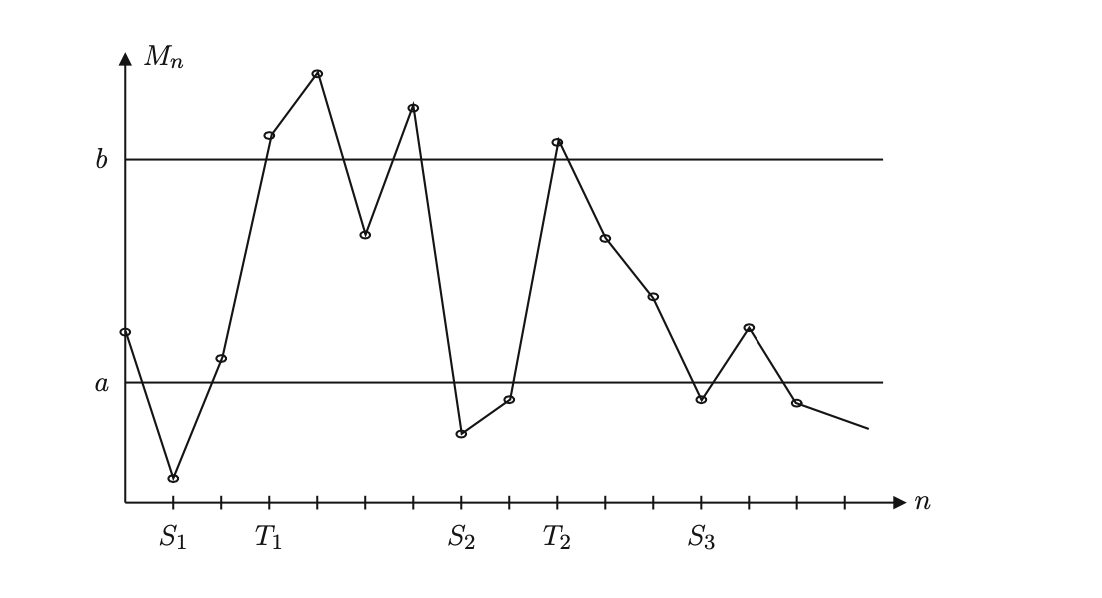
\includegraphics[scale=0.5]{GY-stat547c/doc/report/upcrossing.png}
  \caption{Upcrossing Time of (a,b)}
  \label{fig:birds}
\end{figure}
\begin{theorem}{Doob’s Upcrossing Inequality}
If $(X_n, \mathcal{F}_n)$is a submartingale, $a<b$ and $U_n(a,b)$ is the upcrossing number of $[a,b]$, then $$\mathbb{E}U_n(a,b)\le\frac{\mathbb{E}(X_n-a)^+-\mathbb{E}(X_0-a)^{+}}{b-a}$$
\end{theorem}
\begin{proof}
Define $Y_n=a+(X_n-a)^{+}$, then $Y_n$ is a submartingale, and $$(b-a)U_n \le (H \cdot Y)_n.$$ Here we replace $X_n$ with $Y_n$.
Notice that $$Y_n-Y_0=(H \cdot Y)_n+((1-H)\cdot Y)_n$$ From Theorem 2,  $$\mathbb{E}[((1-H)\cdot Y)_n] \ge \mathbb{E}[((1-H)\cdot Y)_0] \implies \mathbb{E}(H \cdot Y)_n \le \mathbb{E}(Y_n-Y_0),$$ which completes the proof.
\end{proof}
here are two things that we need to be meticulous about. First, $Y_n$ is a submartingale because $x \mapsto (x-a)^{+}$ is convex and non-decreasing. Then we can apply Jesen's inequality:
$$\mathbb{E}(\varphi(X_{n+1}|\mathcal{F}_n))\ge \varphi(\mathbb{E}(X_{n+1}|\mathcal{F}_n))\ge \varphi(X_n)$$
In addition, the reason to replace $X_n$ by $Y_n$ is that $Y_n$ upcrosses $(a,b)$ the same number of times as that $X_n$ does, and the final incomplete upcrossing is always non-negative. Therefore, we can use $Y_n$ instead of $X_n$ in the proof.\\\\ 
Hence, we can use Upcrossing Inequality as a tool to prove the Martingale Convergence Theorem 1.

\subsection{Proof of MCT 1}

\begin{proof}
Since $X_n \in L^1$, 
$$\mathbb{E}[X_n^+]\le \mathbb{E}[|X_n|]=2\mathbb{E}[X_n^+]-\mathbb{E}[X_n]\le 2\mathbb{E}[X_n^+]-\mathbb{E}[X_0]$$ and $$\sup_{n}\mathbb{E}[X_n^{+}]<\infty \iff \sum_{n}\mathbb{E}[|X_n|]<\infty$$
Define \begin{align*}
    A &=\{\omega \in \Omega: X_n(\omega)\nrightarrow X(\omega)\}\\&=\{\omega \in \Omega: \lim \inf_{n \to \infty}X_n(\omega)<\lim \sup_{n\to \infty}X(\omega)\}\\&=\bigcup_{a,b\in \mathbb{Q},a<b}\{\omega \in \Omega: \lim \inf_{n \to \infty}X_n(\omega)<a<b<\lim \sup_{n\to \infty}X(\omega)\}
\end{align*}
Also, note that $$\{\omega \in \Omega: \lim \inf_{n \to \infty}X_n(\omega)<a<b<\lim \sup_{n\to \infty}X(\omega)\}\subset\{\omega \in \Omega: U_{\infty}(a,b)(\omega)=\infty\}$$ where $U_{\infty}(a,b)=\lim_n U_n(a,b)$ and $U_n(a,b)$ is the number of upcrossings of$(a,b)$. Apply Monotone Convergence Theorem and Doob’s Upcrossing Inequality, 
$$\mathbb{E}[U_{\infty}(a,b)]=\lim_{n}\mathbb{E}[U_n(a,b)]\le \frac{\sup_n \mathbb{E}[(X_n-a)^{+}]}{b-a}\le \frac{\sup_n \mathbb{E}[X_n^+]+|a|}{b-a}<\infty$$ Also, note that $$\mathbb{E}[U_{\infty}(a,b)]<\infty \implies P(U_{\infty}(a,b)=\infty)=0$$ Observe that the sequence of  sets $\{\omega \in \Omega: \lim \inf_{n \to \infty}X_n(\omega)<a<b<\lim \sup_{n\to \infty}X(\omega)\}$ is countable, $$P(A)\le \sum_{a<b, a,b\in \mathbb{Q}}P\{\omega \in \Omega: \lim \inf_{n \to \infty}X_n(\omega)<a<b<\lim \sup_{n\to \infty}X(\omega)\}=0$$Hence, $$\lim_{n \to \infty}X_n=\lim \sup_{n \to \infty}X_n=\lim \inf_{n \to \infty}X_n=X_{\infty} \ \text{almost surely}.$$ This completes the proof of Martingale Convergence Theorem 1.\end{proof}

Throughout my analysis, I get to appreciate the beauty within this proof as we can regard "not convergence" as an event, and apply Upcrossing Inequality to demonstrate the probability of every single event is 0 then. I feel that whereas mathematicians whose primary focus is analysis incline to think questions from the perspective of probability distributions, mathematicians with a focus on probability tend to tackle identical questions based on events.\\\\
Based on the proof of the Martingale Convergence Theorem (1), I want to leave two exercises, which help understand Martingale Convergence Theorem. The solutions to exercises can be found in the Appendix.
\begin{exercise}
Let $X_n$ be a $(\mathcal{F}_n)$-martingale with bounded increments. Martingale with bounded increments mean that there exists $M>0$ such that $\sup_n |X_{n+1}-X_n|\le M$. Then with probability 1:\begin{itemize}
    \item $\lim \inf_n X_n=-\infty$, $\lim \sup_n X_n=+\infty$
    \item $\lim_n X_n$ exists and it is finite
\end{itemize}
\end{exercise}
\begin{exercise}
Prove the second Borel-Cantelli Lemma: Let $\mathcal{F}_n$ be a filtration. $A_n \in \mathcal{F}_n$ is a sequence of events, Then $$\{A_n \ i.o.\}=\{\omega: \sum_{n=1}^{\infty}P(A_n|\mathcal{F}_{n-1}=\infty)\}$$
\end{exercise}
I am going to introduce the Martingale Convergence Theorem 2, which furthers Martingale Convergence Theorem 1.
\subsection{MCT 2}
\begin{theorem}
Let $X=(X_n, \mathcal{F}_n)_{n \in \mathbb{N}}$ be a martingale. If $(X_n)_{n \in \mathbb{N}}$ is uniformly integrable, then $X_n \to X_{\infty}$ in $L^1$ \textbf{almost surely}. Moreover, $X_n=\mathbb{E}[X_{\infty}|\mathcal{F}_n]$ for all $n \in \mathbb{N}$.
\end{theorem}
\begin{proof}
Recall that a collection of random variables $\{X_i,  i \in I\}$ is uniformly integrable if $$\lim_{M \to \infty}\sup_{i \in I}\mathbb{E}[|X_i|\mathbbm{1}_{\{|X_i|>M\}}]=0$$ and $$\{X_i\}\ \text{is uniformly integrable} \implies \{X_i\} \ \text{is} \ L^1 \ \text{bounded}$$ In addition, if $X_n$  is a submartingale,
the following statements are equivalent:
\begin{itemize}
    \item $\{X_n : n\ge 0\}$ is uniformly integrable.
    \item $X_n \to X_{\infty}$ almost surely and $X \in L^1$
    \item $X_n \to X_{\infty}$ in $L^1$
\end{itemize}
I am not gong to prove the above lemmas because we have already leant in class at a certain point.
Therefore, to prove MCT 2, the only part we left is to show $X_n=\mathbb{E}(X_{\infty}|\mathcal{F}_n)$.\\
Since $X_n \to X_{\infty}$ in $L^1$, we have $$|\mathbb{E}X_m \mathbbm{1}_A-\mathbb{E}X_{\infty} \mathbbm{1}_A|\le \mathbb{E}|X_m\mathbbm{1}_A-X_{\infty}\mathbbm{1}_A|\le \mathbb{E}|X_m-X_{\infty}|\to 0$$Therefore, $$\mathbb{E}(X_m \mathbbm{1}_A) \to \mathbb{E}( X_{\infty}\mathbbm{1}_A)$$ Since $(X_n,\mathcal{F}_n)$ is a martingale, $\mathbb{E}(X_m|\mathcal{F}_n)=X_n, \forall m>n$, and it implies that $$\mathbb{E}(X_n \mathbbm{1}_A)=\mathbb{E}[X_m\mathbbm{1}_{A}]$$
Recall that $\mathbb{E}(X_m \mathbbm{1}_A) \to \mathbb{E}( X_{\infty}\mathbbm{1}_A)$, we can get that $$\mathbb{E}[X_n\mathbbm{1}_A]=\mathbb{E}[X_{\infty}\mathbbm{1}_A], \forall A\in \mathcal{F}$$ Therefore,  $$\mathbb{E}[{X_{\infty}|\mathcal{F}_n}]=X_n$$
\end{proof}
Overall, the proof of second Martingale Convergence Theorem is more about the understanding of martingale properties and the equivalence of the three properties of martingales: (i) uniformly integrable, (ii) convergence almost surely and in $L^1$, (iii) convergence in $L^1$.  

\subsection{Doob’s Martingale Inequality}
\begin{theorem}
If $X=(X_n, \mathcal{F}_n)_{n \in \mathbb{N}}$ is a martingale in $L^p$, where $p \ge 1$. Then for $c>0$,
$$P\{\max_{k \le n}|X_k|>c\}\le \frac{1}{c^p}\mathbb{E}[|X_n|^p]$$ 
\end{theorem}
This is a more graceful extended  version of Doob-Kolmogorov inequality, which. is $$P(\max_{1 \le m \le n}X_n \ge c)\le \frac{\mathbb{E}[X_n^2]}{c^2}$$These results are commonly used in Stochastic Optimization problems because in a time interval $[1,n]$, the worst case deviation of a submartingale is proportional to the value of $X_n$. Since these inequalities are widely applied in many stochastic optimization algorithms, I feel the necessity to prove it. To simplify the proof process, I will first prove the Doob-Kolmogorov Inequality, then use the result to show Theorem 5.
\begin{proof}
Define $A=\{\max_{1 \le m \le n}X_m \le c\}$ and $B_m=\{\max_{1 \le i \le m_1}X_i\le c, X_m \ge c\}$.  This can be explained as $B_m$ is the event that the submartingale $X_n$ touches $c$ for the first time at time $m$. It is obvious that the whole space $\Omega=A \cup (\cup_{1\le m \le n} B_m)$, and $A, B_m$ are exclusive, so 
$$\mathbb{E}[X_n^2]=\mathbb{E}[X_n^2 \mathbbm{1}_A]+\sum_{1\le m \le n}\mathbb{E}[X_n^2 \mathbbm{1}_{B_m}]\ge \sum_{1\le m \le n}\mathbb{E}[X_n^2 \mathbbm{1}_{B_m}]$$
Note that \begin{align*}
    \mathbb{E}[X_n^2\mathbbm{1}_{B_m}]&=\mathbb{E}[(X_n-X_m+X_m)^2\mathbbm{1}_{B_m}]\\&=\mathbb{E}[(X_n-X_m)^2\mathbbm{1}_{B_m}]+2\mathbb{E}[(X_n-X_m)X_m\mathbbm{1}_{B_m}]+\mathbb{E}[X_m^2\mathbbm{1}_{B_m}]
\end{align*}
Observe that 
$\mathbb{E}[(X_n-X_m)^2\mathbbm{1}_{B_m}]\ge 0$, and  
$$\mathbb{E}[X_m^2\mathbbm{1}_{B_m}]= X_m^2 \mathbb{E}[\mathbbm{1}_{B_m}]\ge c^2P(B_m)$$ Apply tower property, \begin{align*}
    \mathbb{E}[(X_n-X_m)X_m\mathbbm{1}_{B_m}]&=\mathbb{E}[\mathbb{E}[(X_n-X_m)X_m\mathbbm{1}_{B_m}]|\mathcal{F}_m]\\&=\mathbb{E}[X_m \mathbbm{1}_{B_m}\mathbb{E}[(X_n-X_m)|\mathcal{F}_m]]
\end{align*}
Since $X_n$ is a submartingale, then $\mathbb{E}[(X_n-X_m)|\mathcal{F}_m]]\ge 0$. Since $X_m \mathbbm{1}_{B_m}$ is either 0 or $c>0$, $X_m \mathbbm{1}_{B_m} \ge 0$
So, $$\mathbb{E}[(X_n-X_m)X_m\mathbbm{1}_{B_m}]\ge 0$$
Thus, we can get $$\mathbb{E}[X^2]\ge \sum_{1 \le m \le n}c^2P(B_m)=c^2P(\cup_{m}B_m)=c^2P(\max_{1 \le m \le n}X_m>c)$$ This completes the proof of Doob-Kolmogorov inequality.\\
Now we can use this result to prove the general version. Since  absolute value functions and $f(x)=x^{\frac{p}{2}}$, for $p \ge 2$ are convex functions, applying Jesen's inequality (which can be found in section 2.4), $|X_n|^{\frac{p}{2}}$ is also a submartingale. Thus, $$P(\max_{1 \le m\le n}|X_n|\ge \varepsilon)=P(\max_{1\le m \le n}|X_n|^{\frac{p}{2}}\ge c^{\frac{p}{2}})\le \frac{\mathbb{E}[|X_n|^p]}{c^p}$$
\end{proof}
The idea of this proof is similar to that of Doob's Upcrossing Inequality. The first and foremost step is to construct the events $A$ and $B$, which work to describe the relationship between submartingale $X_n$ and time $m$. As subsets of sample space, the expected values can be connected with probability through indicator functions. Jesen's inequality of martingales plays a crucial role in this proof as well. It is a useful tool in martingale proof and optimization problems since it simplifies the originally complicated process of proof, as illustrated when demonstrating the general case of Doob's Martingale Inequality.

\section{Related Research: Robbins-Siegmund Theorem}
In this section, I am going to introduce Stochastic Optimization briefly and discuss the application of Martingale Convergence Theorem in Robbins-Siegmund Theorem.\\\\
Stochastic Optimization aims to find an optimal solution to a problem by minimizing or maximizing an objective function with randomness. It plays a crucial role in Machine Learning. Martingales are usually applied to Stochastic Optimization algorithms due to their corresponding properties. Robbins-Siegmund Theorem is one of the most valuable results in Stochastic algorithms, because it can be applied to convergence of the stochastic gradient method.  Martingale Convergence Theorem plays a significant role in the proof of Robbins-Siegmund Theorem \cite{S.Gadat:2018}.
\begin{theorem}{Robbins-Siegmund}
 $(\mathcal{F}_n)_{n \ge 0}$ is a filtration. The four random variables $(U_n)$, $(V_n)$, $(\alpha_n)$ and $(\beta_n)$ are $(\mathcal{F}_n)$-measurable, non-negative, integrable and satisfy the following properties:
 \begin{itemize}
     \item $(U_n)$, $(\alpha_n)$ and $(\beta_n)$ are $(\mathcal{F}_n)$-predictable
     \item $\sup_{\omega \in \Omega}\prod_{n \ge 1}(1+\alpha_n(\omega))<\infty$ and $\sum_{n \ge 0}\mathbb{E}[\beta_n]<\infty$
     \item $\forall n \in \mathbb{N}$, $\mathbb{E}[V_{n+1}|\mathcal{F}_n]\le V_n(1+\alpha_{n+1})+\beta_{n+1}-U_{n+1}$
 \end{itemize}
 Then we can get the following two results:
 \begin{enumerate}
     \item $V_n \to V_{\infty} \in L^1$ and $\sup_{n \ge 0}\mathbb{E}[V_n]<\infty$
     \item $\sum_{n \ge 0}\mathbb{E}[U_n]<\infty$ and $\sum_{n \ge 0}U_n<\infty$
 \end{enumerate}
 
\end{theorem}
\begin{proof}
Since $U_n$ is predictable and the four variables are all non-neagtive,
\begin{align*}
    \mathbb{E}\left(V_{n+1}+\sum_{k=1}^{n+1}U_k\left.\right|\mathcal{F}_n\right) &\le V_n(1+\alpha_{n+1})+\sum_{k=1}^{n}U_k+\beta_{n+1}\\&\le \left(V_n+\sum_{k=1}^{n}U_k\right)(1+\alpha_{n+1})+\beta_{n+1}
\end{align*}
Divide $\prod_{k=1}^{n+1}(1+\alpha_k)$ to both sides:
$$\mathbb{E}\left(\frac{V_{n+1}+\sum_{k=1}^{n+1}U_k}{\prod_{k=1}^{n}(1+\alpha_k)}\left.\right|\mathcal{F}_n\right) \le \frac{\left(V_n+\sum_{k=1}^{n}U_k\right)(1+\alpha_{n+1})}{\prod_{k=1}^{n+1}(1+\alpha_k)}+\frac{\beta_{n+1}}{\prod_{k=1}^{n+1}(1+\alpha_k)}$$
We can obtain $$\mathbb{E}[S_{n+1}|\mathcal{F}_n]\le S_n +\tilde{\beta}_{n+1}$$ where $$S_n=\frac{V_n+\sum_{k=1}^{n}U_k}{\prod_{k=1}^{n}(1+\alpha_k)}, \ \tilde{\beta}_n=\frac{\beta_n}{\prod_{k=1}^{n}(1+\alpha_k)}$$ Define $B_n=\sum_{k=1}^{n}\tilde{\beta}_k.$ Since $$\sup_{\omega \in. \Omega}\prod_{n \ge 1}(1+\alpha_n(\omega))<\infty, \ \beta_n \text{is integrable},$$ we can obtain that $$B_n \to B_{\infty} \ \text{almost surely and } B_{\infty}\in L^1 \implies \mathbb{E}B_{\infty}<\infty$$ In addition, 
$$\sum_{n \ge 0}\mathbb{E}[\beta_n]<\infty \implies \sup_{n \ge 0}\mathbb{E}[S_n]<\infty$$
The next step is to \textbf{construct a super-martingale}. Define $\tilde{S}_n=S_n+\mathbb{E}[B_{\infty}|\mathcal{F}_n]-B_n$. We need to show$\tilde{S}_n$ is a supermartingale. Since $\mathbb{E}[S_{n+1}|\mathcal{F}_n]\le S_n+\tilde{\beta}_{n+1}$ and $B_n \to B_{\infty}$, then \begin{align*}
   \mathbb{E}[\tilde{S}_{n}|\mathcal{F}_n] &\le  S_n+\tilde{\beta}_{n+1}+\mathbb{E}[B_{\infty}|\mathcal{F}_n]-\mathbb{E}[B_{n+1}|\mathcal{F}_n]\\& \le S_n+\mathbb{E}[B_{\infty}|\mathcal{F}_n]-B_{n+1}+\tilde{\beta}_{n+1}\\&=\tilde{S}_n
\end{align*} 
Check $\tilde{S}_n\in L^1$: $$\mathbb{E}|\tilde{S}_n|\le \mathbb{E}(|S_n|+|\mathbb{E}[B_{\infty}|\mathcal{F}_n]-B_n|)\le \mathbb{E}S_n+\mathbb{E}B_{\infty}<\infty$$
Therefore, $(\tilde{S}_n)$ is a super-martingale. Apply \textbf{Martingale Convergence Theorem}, 
$$\tilde{S}_n \to \tilde{S}_{\infty} \ \text{and} \ \tilde{S}_{\infty}\in L^1$$
Since $\mathbb{E}[B_{\infty}|\mathcal{F}_n]-B_n \to 0$, in fact $S_{\infty}=\tilde{S}_{\infty}$ and $S_{\infty}\in L^1$. Also  $$S_n\le \tilde{S}_n \implies \sup_{n \ge1}\mathbb{E}[S_n]<\mathbb{E}[\tilde{S}_n]<\infty$$ Recall that $$S_n=\frac{V_n+\sum_{k=1}^{n}U_k}{\prod_{k=1}^{n}(1+\alpha_k)} \implies \mathbb{E}[V_n]+\mathbb{E}\left(\sum_{k=1}^{n}U_k\right)=\mathbb{E}[\left(\prod_{k=1}^{n}(1+\alpha_K)\right)S_n]$$
Since $$\mathbb{E}[\left(\prod_{k=1}^{n}(1+\alpha_K)\right)S_n]\le \left \lVert \prod_{k=1}^{\infty}(1+\alpha_k)\right \rVert_{\infty}\mathbb{E}[S_n]<\infty$$
Therefore, $$\sup_{n \ge 1}\mathbb{E}[V_n]<\infty$$ and $$\mathbb{E}[\sum_{k \ge 1}U_k]<\infty \implies \sum_{k \ge 1}U_k<\infty \ \text{almost surely}$$ Recall that $S_n \to S_{\infty}$ and $\prod_{k \ge 1}(1+\alpha_k)<\infty$, $$V_n=S_n\prod_{k\ge 1}^{n}(1+\alpha_k)-\sum_{k \ge 1}U_k \to S_{\infty}\prod_{k \ge 1}(1+\alpha_k)-\sum_{k \ge 1}U_k=V_{\infty} \in L^1\ \text{almost surely}$$
This completes the proof.
\end{proof}
The most critical step in this proof of the Robbins-Siegmund Theorem is to construct super martingales with some given properties of random variables, then rearrange them and apply Martingale Convergence Theorem to  $\tilde{S}_n, S_n $and $B_n $ several times. This step brings significant convenience when proving the convergence of stochastic optimization algorithms. For instance, the key idea of the proof of De Finetti’s Theorem\cite{David:2013} (Given a sequence of exchangeable, tat is, for any $\pi_n \in S_n, (X_1, \cdots, X_n)\overset{\Delta}{=}(X_{\pi_n(1)},\cdots, X_{\pi_n(n)})$, then conditional on $\xi$, $X_1, \cdots, X_n$  are i.i.d.) is to construct martingales and appy backward MG convergence theorem. \\\\
In \cite{pmlr-v99-anastasiou19a}, Andreas, Krishnakumar and Murat (2019) provided non-asymptotic convergence rates of the Polyak-Ruppert averaged stochastic gradient descent (SGD) to a normal random vector with Martingale Central Limit Theorem, which is an extended version of Martingale Convergence Theorem. This paper \cite{Zhengyuan:etal}discssed  the convergence of mirror descent in a class of stochastic optimization problems which are variational coherence by constructing submartingales combined with a series of submartingale convergence arguments. In general, the usage of Martingale Convergence Theorem brings insights to proving convergence in stochastic optimization problems.  By employing this brilliant theory, we can tackle the problems of convergence rate with much ease.




% background section

\section{Acknowledgement}
I want to thank for Anqi Pu for helping me correct my grammatical mistakes and navigate through scientific writing. I also want to thank Yuchong Pan and David Xu who gave me a lot of valuable advice on my project. 

% add your main body sections here

% open questions section
\newpage
\printbibliography
%%%% appendix
\clearpage

\appendix

% exercises and problems
% !TEX root = ../main.tex

% Exercises section

\section{Exercises}
\begin{enumerate}
    \item 

Let $X_n$ be a $(\mathcal{F}_n)$-martingale with bounded increments. Note that Martingale with bounded increments mean that there exists $M>0$ such that $\sup_n |X_{n+1}-X_n|\le M$. Then with probability 1:\begin{itemize}
    \item $\lim \inf_n X_n=-\infty$, $\lim \sup_n X_n=+\infty$
    \item $\lim_n X_n$ exists and it is finite
\end{itemize}

\begin{proof}
Without loss of general, pick $X_0=0$ by replacing $X_n$ with $X_n-X_0$. Let $N_k=\inf\{n:X_n\ge k\}, k>0$, then $N_k$ is a stopping time by checking $\{N_k \le n\}\in \mathcal{F}_n$. Therefore, by Corollary 1, $X_{n\wedge N_k}$ is a martingale, and $$0\le (X_{n\wedge N_k})^{+}\le k+M, \ \forall n \in \mathbb{N}$$ due to the way we define $N_k$ and the definition of bounded on increments. Therefore, $$\mathbb{E}[(X_{n\wedge N_k})^{+}]\le k+M<\infty \implies \lim_{n \to \infty}X_{n \wedge N_k}\ \text{exists and is finite }$$ Then by Martingale Convergence Theorem, $$\lim_{n \to \infty}X_n=\lim_{n \to \infty}X_{n \wedge N_K}  \ \text{exists almost surely and is finite}$$ In other words, $X_n\mathbbm{1}_{\{N_k=\infty\}}$ converges almost surely. Then for $$\omega  \in \bigcup_{k \in \mathbb{N}}\{N_k=+\infty\}=\{\lim \sup_{n \to \infty}X_n<\infty\} \ (\text{real analysis )}$$
Thus, $\lim_{n \to \infty}X_n$ exists and is finite. Replacing $X$ with $-X$, then for almost every $\omega \in \{\lim \inf_{n \to \infty}X_n>-\infty\}$, $\lim_{n \to \infty}X_n$ exists and is finite. Let $$C=\{\lim_{n \to \infty}X_n \ \text{exists and is finite}\}$$, $$D=\{\{\lim \sup_{n \to \infty}X_n<\infty\}\cup \{\lim \inf_{n \to \infty} X_n>-\infty\}\}$$
We have shown that $D \subset C$, then $$P(D \cap C^c)=0 \implies P(D^c \cup C)=1 \ \text{almost surely}$$
$D^c$ is the first property and C is the second property, this completes the proof

\end{proof}
\item Proof the Second Borel-Cantelli Lemma
\begin{proof}
Construct a martingae $$M_n=\sum_{k=1}^n(\mathbbm{1}_{A_k}-P(A_k|\mathcal{F}_{k-1}))$$ where $|M_n|\le n, \forall n$ and $|M_{n+1}-M_n|\le 1, \forall n$.
Using the same notation as what we used in the proof of Exercise 1, On $C=\{\lim_{n \to \infty}X_n \ \text{exists and is finite}\}$, we have $$\sum_{k=1}^{\infty}\mathbbm{1}_{A_k}=+\infty \iff \sum_{k=1}^{\infty}P(A_k|\mathcal{F}k)=\infty$$ This is because if either $$\sum_{k=1}^{\infty}\mathbbm{1}_{A_k}<\infty \ \text{or}\ \sum_{k=1}^{\infty}P(A_k|\mathcal{F}_{k-1})<\infty,$$ then $$M_n \to \left(\sum_{k=1}^{\infty}\mathbbm{1}_{A_k}\right)-\left(\sum_{k=1}^{\infty}P(A_k|\mathcal{F_{k-1}})\right)>\infty$$
On $D^c=\{\{\lim \sup_{n \to \infty}X_n=\infty\}\cup \{\lim \inf_{n \to \infty} X_n=-\infty\}\}$, we have $$\sum_{n=1}^{\infty}\mathbbm{1}_{A_n}=\infty \ \text{and} \sum_{n=1}^{\infty}P(A_n|\mathcal{F}_{n-1})=\infty$$
This completes the proof.
\end{proof}

% any other appendix sections

\end{enumerate}
% bibliography


\end{document}